\documentclass[letterpaper, 12pt]{article}
\usepackage[letterpaper, top=2.5cm, bottom=2.5cm, left=3cm, right=3cm]{geometry} %margenes
\usepackage[utf8]{inputenc} %manejo de caracteres especiales
\usepackage[spanish]{babel} %manejo de encabezados de inglés a español
\usepackage{fancyhdr} %formato de los encabezados de página
\usepackage{ragged2e} %alineado real justficado
\usepackage{graphicx} %manejo de imagenes
\usepackage{amsmath} %manejo de notación matemática
\usepackage{mathtools} %manejo de notación matemática
\usepackage{blindtext} %texto de relleno
\usepackage{cancel} %permite la simbolización de cancelación de terminos
\usepackage{enumitem}[shortlabels] %listas con letras
\usepackage{amssymb} %manejo de simbolog►1a matematica

\pagestyle{fancy}
\fancyhf{}
\rfoot{\thepage}

\begin{document}

\setcounter{page}{1}
\thispagestyle{fancy}
\lhead{\textbf{Tarea 2, U1}}
\rhead{\textbf{18/09/2020}}
\section{Vectores en el espacio}
\subsection*{Resolver las siguientes operaciones: (\(\vec{u}+\vec{w},\,\vec{v}-\vec{u},\,\vec{w}-5\vec{v},\,3\vec{u}+\vec{v},\,\lambda\vec{u},\,\lambda\vec{w}\)) y graficar a mano los vectores:}
\begin{itemize}
    \item \(\vec{u}=<4,5>\)
    \item \(\vec{v}=\hat{i}+3\vec{j}\)
    \item \(\vec{w}=<-4,-1>\)
\end{itemize}
xd
\subsubsection*{-Gráfica de los vectores:}
\centering
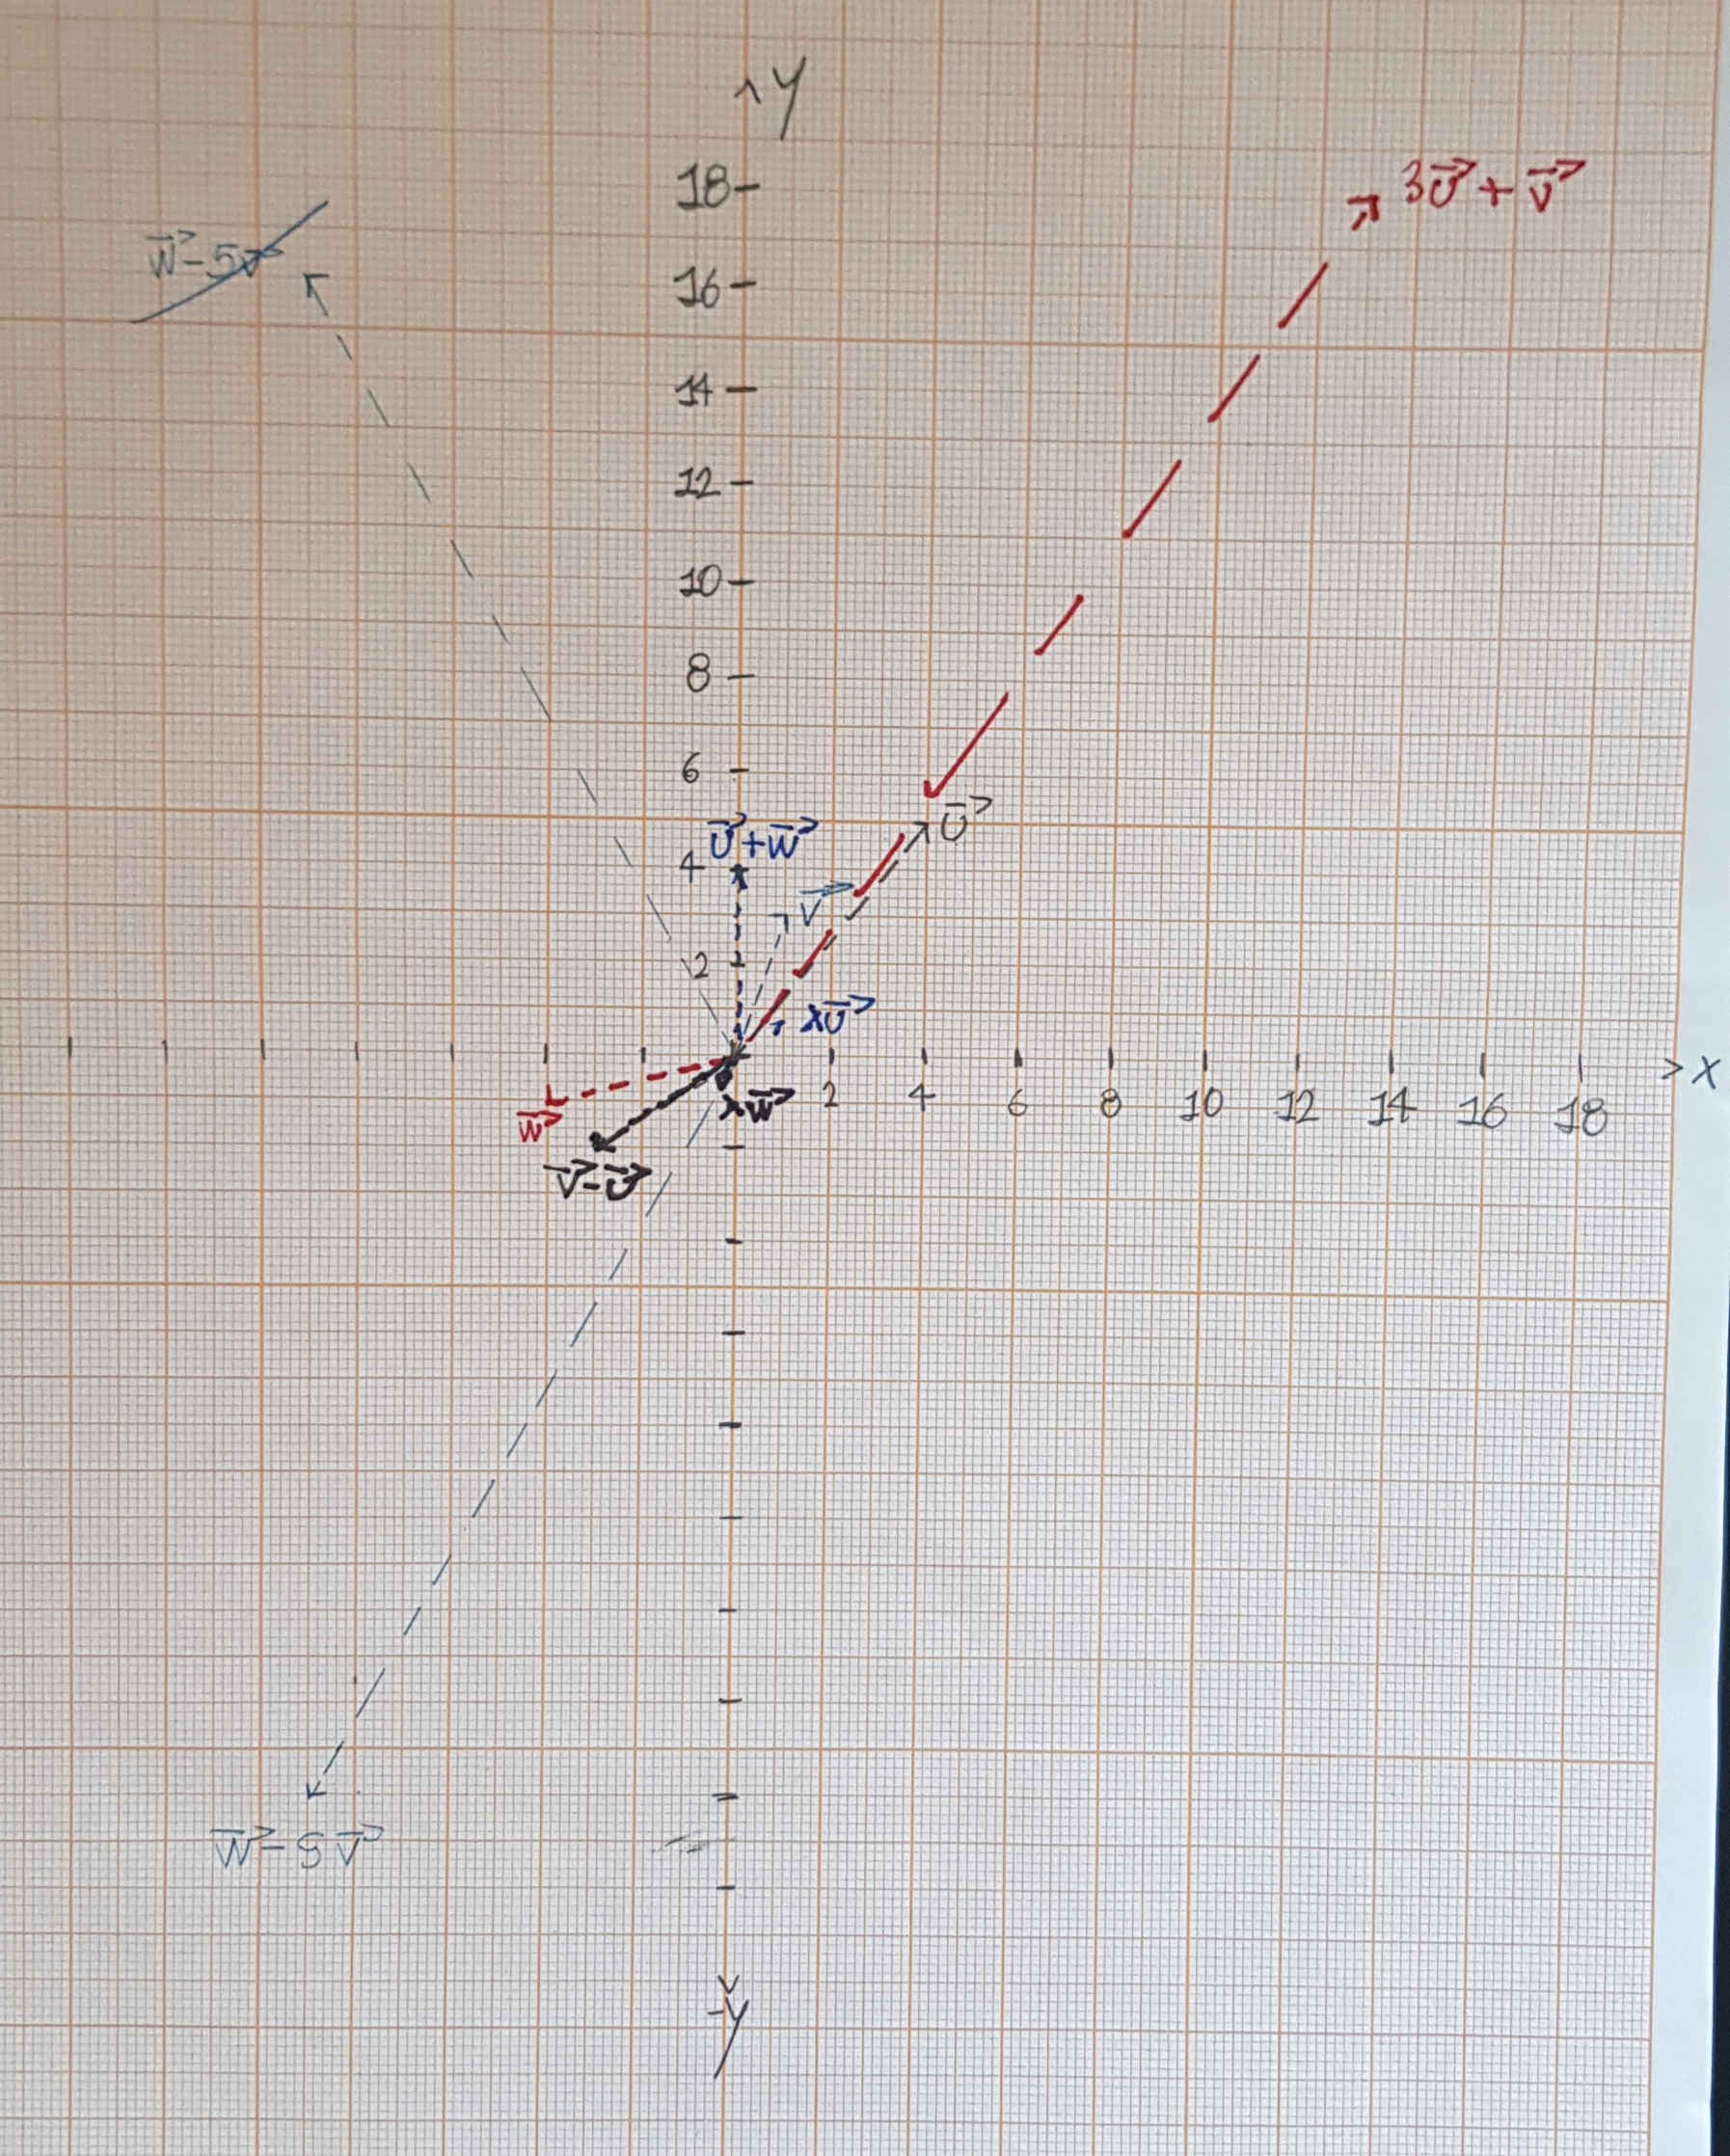
\includegraphics[width=12cm,]{grafica.jpg}
\justify
\begin{align*}
\textbf{Operaciones:}\\ \text{\newline}
\vec{u}+\vec{w}=&<4,5>+<-4,-1>\,=\,<4-4,5-1>\,=\,<0,4>;\\
\vec{v}-\vec{u}=&<1,3>-<4,5>\,=\,<1-4,3-5>\,=\,<-3,-2>;\\
\vec{w}-5\vec{v}=&<-4,-1>-\,5\,\cdot<1,3>\,=\,<-4,-1>-<5\cdot 1,5\cdot 3>\,=
\\<-4,-1>&\,-<5,15>\,=\,<-4-5,-1-15>\,=\,<-9,-16>;\\
3\vec{u}+\vec{v}=&\,3\,\cdot<4,5>+<1,3>\,=\,<3\cdot 4,3\cdot 5>+<1,3>\,=
\\<12,15>&\,+<1,3>\,=\,<12+1,15+3>\,=\,<13,18>;\\
\lambda\vec{u}=\frac{\vec{u}}{\|\vec{u}\|};\,&\|\vec{u}\|=\sqrt{u_1^2+u_2^2}=\sqrt{4^2+5^2}=\sqrt{16+25}=\sqrt{41}\,\therefore\,\lambda\vec{u}=\frac{<4,5>}{\sqrt{41}}=\\
<\frac{4}{\sqrt{41}},\frac{5}{\sqrt{41}}>;\\
\lambda\vec{w}=\frac{\vec{w}}{\|\vec{w}\|};\,&\|\vec{w}\|=\sqrt{w_1^2+w_2^2}=\sqrt{(-4)^2+(-1)^2}=\sqrt{16+1}=\sqrt{17}\,\therefore\,\lambda\vec{u}=\frac{<-4,-1>}{\sqrt{17}}=\\
<\frac{-4}{\sqrt{17}},\frac{-1}{\sqrt{17}}>;\\
\end{align*}

\end{document}